\documentclass[12pt]{article}
\usepackage[utf8]{inputenc}
\usepackage{graphicx} 
\usepackage[dvipsnames]{xcolor}
\usepackage{moreverb}
\renewcommand\refname{Referencias}
\title{Elementos de la programación Python 1.}
\author{\textcolor{JungleGreen}{Olga María Fimbres Morales}}
\date{28 de Enero 2016}
\begin{document}
\begin{titlepage}

\begin{center}
\begin{large}
Universidad del Estado de Sonora\\
\end{large}
\vspace*{0.15in}
División de Ciencias Exactas y Naturales.\\
\vspace*{0.15in}
Licenciatura en Física. \\
\vspace*{0.6in}
\begin{large}
Física Computacional 1\\
\end{large}
\vspace*{0.2in}
\begin{Large}
\textbf{{\textcolor{Red}{Ajuste de datos.}}} \\
\end{Large}
\vspace*{0.3in}
\begin{large}
\textbf{{\textcolor{Green}{Ajuste de mínimos cuadrados.}}} \\
\end{large}
%\vspace*{-1in}

\rule{80mm}{0.1mm}\\
\vspace*{0.1in}
\begin{large}
{\textcolor{JungleGreen}{Olga María Fimbres Morales}}\\
21 de Febrero de 2016\\
\end{large}
\end{center}
\end{titlepage}

\pagebreak
\section*{Introducción.}
Durante la realización de algún experimento, o bien durante la recolección de datos sobre algún fenómeno que se este estudiando estos no parecen, en una primera revisión, describir alguna función que podamos expresar adecuadamente de forma matemática.\\
Debido a esto, que resulta muy común en la práctica, es que se han desarrollado diferentes herramientas que nos ayuden en el análisis de los datos y que también nos permitan comprender como estos pueden comportarse en un periodo de tiempo mayor al observado.\\
Dichas herramientas se conocen como análisis de regresión, el cual resulta una gran ayuda al momento de querer comprender el comportamiento de un evento; siendo sumamente importante para aquellos que trabajan en este tipo de situaciones, ya que como sabemos, podemos poseer múltiples modelos que describan una gran variedad de situaciones, pero al momento de estudiar la naturaleza, esta difícilmente se comportara como ya lo hemos estimado.\\
Es por ello que surge la necesidad de este tipo de análisis, y en el presente trabajo se mostrara la forma en que estos trabajan y lo importante que resulta el conocer la forma en como tienden a comportarse los datos para poder realizar una buena decisión al momento de decidir el modelo que se utilizara en el análisis de los datos.\cite{1}
 
\section*{\textcolor{Red}{Regresión lineal y no lineal}}
Una regresión lineal es aquella donde la variable dependiente, $y$, es una combinación lineal de los parámetros; existen diversas formas de realizar esta regresión, pero una de las más utilizadas, que sera la que utilizaremos para este trabajo, sera el de mínimos cuadrados, donde utilizando los datos obtenidos es posible adecuar una recta que pueda utilizarse para describir el fenómenos de una forma adecuada; cabe señalar que no siempre resulta adecuado utilizarla para todo conjunto de datos, ya que podríamos estar realizando una muy mala aproximación que en lugar de facilitar nuestro trabajo solamente lo complicaría más al no permitir una buena descripción de los mismos.\cite{1}\\
Por otro lado, también existen las no lineales, las cuales se basan en datos multidimensionales $x$ y $y$, donde ambos depende de una función $f$ no lineal respecto a algún parámetro desconocido $\theta$; igualmente, se presente obtener los valores de los parámetros asociados a la curva que mejor se ajuste a nuestros datos. Durante nuestro análisis utilizaremos el ajuste exponencial, para lo cual también debemos de tener en cuenta la forma en que se están comportando nuestros datos, ya que de otro modo utilizar esta regresión seria simplemente inútil e innecesario.\cite{2}
\pagebreak
\section*{\textcolor{LimeGreen}{Problema.}}
En el desarrollo de esta actividad se nos han proporcionado una seria de ejemplos donde por medio de la generación de datos aleatorios se adecua una regresión, ya sea lineal o exponencial, permitiendo observar como es que Phyton trabaja con estas herramientas, ya que simplemente ya las tiene programadas en sus bibliotecas, permitiéndonos hacer uso de ellas para una mejor análisis de nuestros datos.\\
Lo que se nos pide realizar a partir de estos ejemplos es la adecuación de cada uno de estas regresiones a unas series de datos que se nos proporcionan sobre distintos fenómenos reales.
\subsection*{Ejejmplo 1.}
\begin{verbatim}
f = np.poly1d([5, 1])

x = np.linspace(0, 10, 30)
y = f(x) + 6*np.random.normal(size=len(x))
xn = np.linspace(0, 10, 200)

plt.plot(x, y, 'or')
plt.show()

m, c = np.polyfit(x, y, 1)
yn = np.polyval([m, c], xn)

plt.plot(x, y, 'or')
plt.plot(xn, yn)
plt.show()
\end{verbatim}
Este código, como ya se mencionó, primeramente realiza una seria de datos aleatorios para después realizar una regresión lineal a partir de los mismos. Dando como resultado la siguiente gŕafica:\\
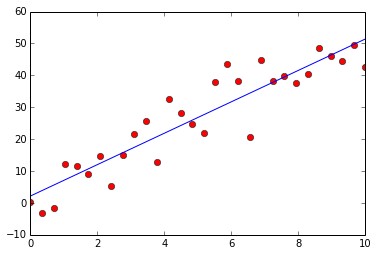
\includegraphics{4c.png}

\subsection*{Ejemplo 2}
\begin{verbatim}
import numpy as np
import matplotlib.pyplot as plt
from scipy.optimize import curve_fit
def func(x, a, b, c):
    return a * np.exp(-b * x) + c

x = np.linspace(0,4,50)
y = func(x, 2.5, 1.3, 0.5)
yn = y + 0.2*np.random.normal(size=len(x))

popt, pcov = curve_fit(func, x, yn)

plt.figure()
plt.plot(x, yn, 'ko', label="Original Noised Data")
plt.plot(x, func(x, *popt), 'r-', label="Fitted Curve")
plt.legend()
plt.show()
\end{verbatim}

El cual realiza la misma operación que el primero, a diferencia que este utiliza una regresión no lineal, adecuando así un ajuste exponencial a los datos:
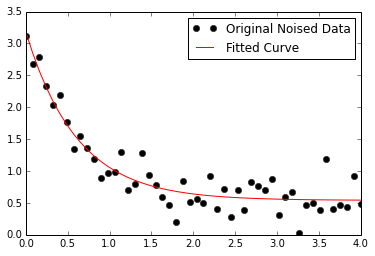
\includegraphics{4d.png}
\pagebreak
\section*{\textcolor{RoyalBlue}{Problema 1}}
Para la primera actividad de nos dio una seria de datos referentes a la temperatura en diversos años del invierno en la ciudad de Nueva York. Se realizó el siguiente código utilizando dichos datos:
\begin{center}
\begin{boxedverbatim}
import matplotlib.pyplot as plt 
import numpy as np

plt.plotfile('act.txt', delimiter=' ', cols=(0, 1), 
             names=('Year', 'Temperature'), marker='o') 
plt.grid(True)

data = np.loadtxt('act.txt')

x1=data[:,0] 
y1=data[:,1] 

#‎Conviert elos arreglos en datos flotantes
x11 = x1.astype(np.float)
y11 = y1.astype(np.float)

xn = np.linspace(1900, 2000, 200)
m, c = np.polyfit(x11, y11, 1)
yn = np.polyval([m, c], xn)

plt.figure()
plt.plot(x11, y11, 'or', label="Datos Originales")
plt.plot(xn, yn, label="Curva Ajustada")
plt.legend()
plt.grid(True)
plt.show()

\end{boxedverbatim}
\end{center}

Nótese que los datos se encontraban en un archivo $.txt$ de donde fue necesario leerlos y una vez que se definió cada columna del archivo como una variable fue necesario convertir esos arreglos a datos flotantes de forma que el código fuera capaz de trabajar con ellos y realizar las distintas operaciones que resultaran necesarias. Puede verse que la parte que realiza la regresión lineal a los datos fue tomada prácticamente igual del ejemplo, siendo únicamente necesario adecuar el rango de esta y adecuando las variables a las que nosotros habíamos utilizado para ubicar nuestros datos.\\
Puede resaltarse que el código posee dos partes donde se realiza la gráfica de datos, siendo la primera una gráfica únicamente de los datos que obtenemos del archivo y la segunda una gráfica de los datos junto con la regresión lineal de los mismos, permitiéndonos de ese modo evaluar si esta resulta confiable o no. De este modo se obtiene las siguientes gráficas como resultados:

\begin{center}
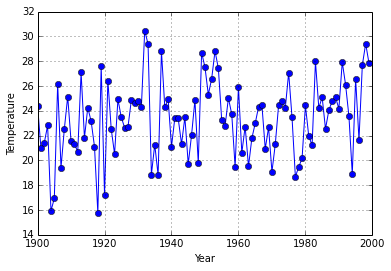
\includegraphics{4a.png}
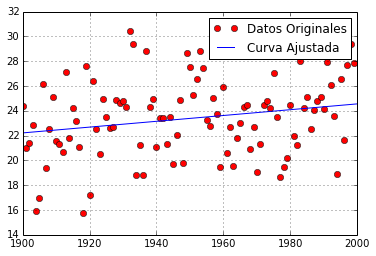
\includegraphics{4aa.png}
\end{center}
\pagebreak
\section*{\textcolor{RoyalBlue}{Problema 2}}
En la segunda actividad se nos proporciona un archivo que contiene datos sobre presión atmosférica y altitud, realizando el segundo código de la siguiente forma:
\begin{center}
\begin{boxedverbatim}
import numpy as np
import matplotlib.pyplot as plt
from scipy.optimize import curve_fit

plt.plotfile('actb.txt', delimiter=' ', cols=(0, 1), 
             names=('Presion', 'Altitud'), marker='o')
plt.grid(True)

data = np.loadtxt('actb.txt')

x1=data[:,0] 
y1=data[:,1] 


#‎Convert‬ array of strings to float
x11 = x1.astype(np.float)
y11 = y1.astype(np.float)

def func(x, a, b, c):
    return a * np.exp(-b * x) + c


yn = y11 + 0.2*np.random.normal(size=len(x11))

popt, pcov = curve_fit(func, x11, yn)

plt.figure()
plt.plot(x11, yn, 'or', label="Datos Originales")
plt.plot(x11, func(x11, *popt), label="Curva Ajustada")
plt.legend()
plt.grid(True)
plt.show()
\end{boxedverbatim}
\end{center}
Nuevamente tras realizar la lectura de los datos y proporcionarle a cada una de las columnas una variable, estos arreglos fueron transformados a datos flotantes, tal como en el código anterior.\\ 
Y de igual modo puede verse que la parte del código que permite el ajuste exponencial fue tomado íntegramente del ejemplo que se nos promocionó al inicio de la actividad, siendo únicamente necesario cambiar las variables por aquellas que estuviéramos utilizando.\\
Para finalmente realizar ambas gráficas de forma que pudiéramos tonar la diferencia de los datos con la regresión que se le aplicó. Las gráficas que se obtuvieron fueron las siguientes:

\begin{center}
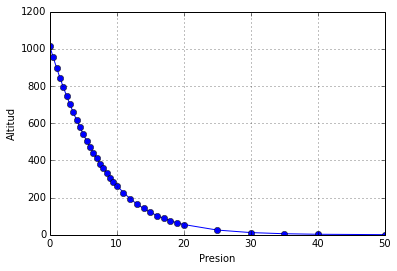
\includegraphics{4b.png}
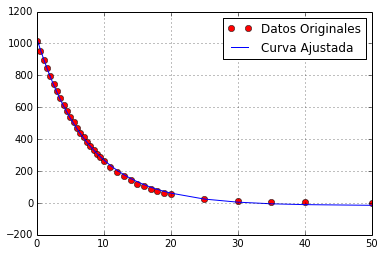
\includegraphics{4bb.png}
\end{center}
\pagebreak


\pagebreak

\begin{thebibliography}{X}
 \bibitem{1} \textsc{Wikipedia, The free encyclopedia; "Regression analysis"; 2016}
 \bibitem{2} \textsc{Wikipedia, The free encyclopedia; "Nonlinear regression"; 2016}
 
\end{thebibliography}
\end{document}